\section{Temporal Mining Mixture Model}
We use a three-pronged approach to tackle the problem of mining and predicting unoccupancy, as 
shown in Figure~\ref{fig_framework}.
\begin{figure}[h]
\centering
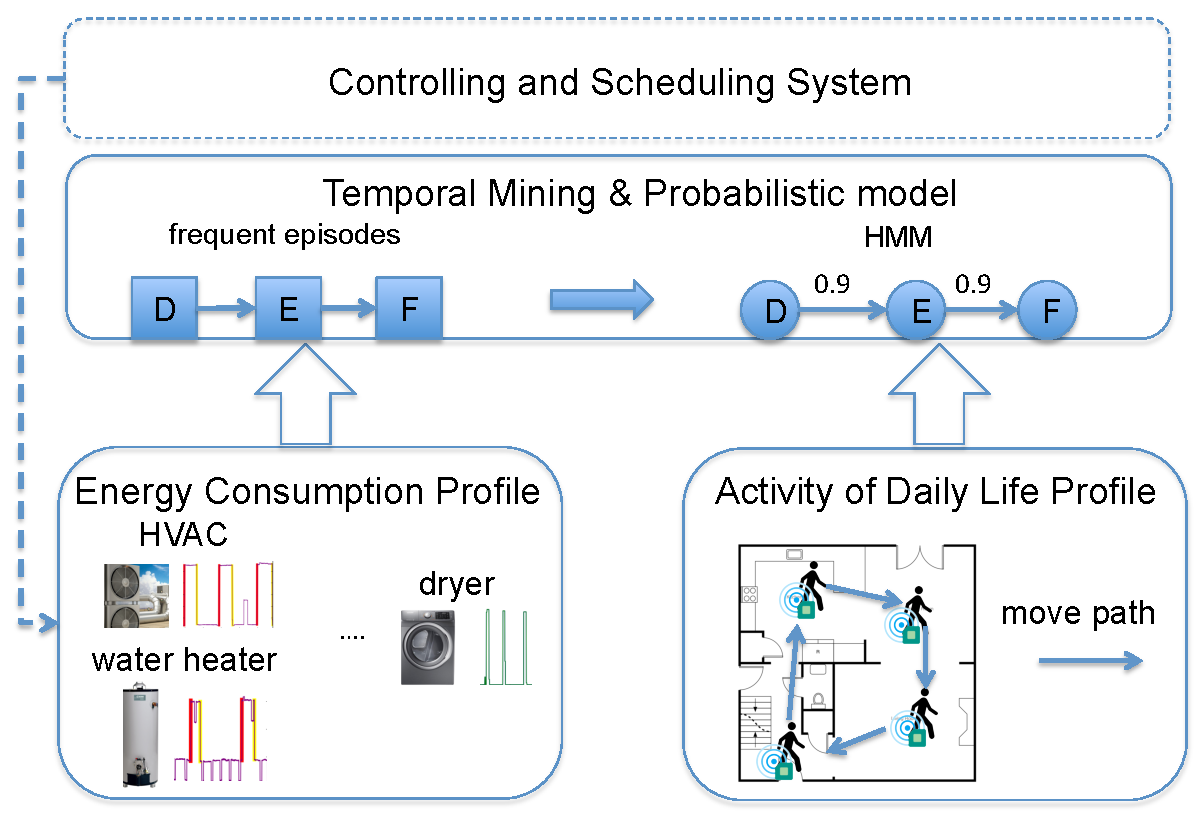
\includegraphics[width=0.5\textwidth]{adlfigs/framework.pdf}
\caption{Occupancy Prediction Framework.\label{fig_framework}}
\end{figure}
Given a time series representing the indoor activities of a person over a period of time, 
first, we use an episode mining algorithm to discover frequent episodes from previous days' data, enabling us to connect each episode with an EGH and build a mixture EGH model. 
Based on this mixture model, we can now predict when each person will leave and return to the house. 
If all the people leave, then the house is unoccupied. 

%Before formalizing the problem statement, we introduce several concepts and notations. 

\textit{Episode} 
An episode is a collection of ordered events. 
Here an episode refers to a set of ordered events which are 
highly relevant to the occupancy status inside a building. 
For instance, let us represent 'S' as sleep, 
'K' as kitchen, and 'Z' as going out. 
If an episode $S \rightarrow K \rightarrow Z$ is found, 
this can be interpreted as a person getting up, 
going to the kitchen for breakfast, and then leaving the house. 
An episode $\alpha$ is composed 
of a series of ordered events
$\alpha=\langle X_1,..,X_t,...X_T \rangle$, 
where $X_t$ denotes that $X$ occurs at a sequence time of $t$.  
The event $X_t$ may be a point event or extend over a longer time, 
in which case it is referred to as a dwelling event with a start time $X.start$ and end time $X.end$. 
In this paper, $X$ denotes a dwelling event and 
indicates the room where a person is located
inside the building, i.e., this building is \emph{occupied}. 
Since $Z$ denotes that a room is unoccupied, 
$Z.start$ is the point at which a person or all the people inside the building leave, and 
$Z.end$ is the point at which one or more of the people come back. 

%\textit{EGH} Episode generative HMM model is a 
%type of HMM model which connects each episode $\alpha$ 
%with a special HMM model $\Lambda_\alpha$. 
%The uniqueness of the EGH is that 
%the transition matrix and 
%emission matrix is only decided by a noise parameter $\eta$. 
%The value of $\eta$ is computed based on the frequency of the 
%corresponding episode $\alpha$. 

\subsection{Time-gap Constraint Episode Mining}
\textbf{Episode Mining}
Episode mining~\cite{mannila1997discovery} uses a non-overlap mining approach to identify frequent episodes. 
It has been applied to energy disaggregation to help conserve energy in buildings~\cite{shao2013temporal} in sustainability research. 
However, in contrast with previous research, 
the events in the current application of occupancy prediction take into account the
dwell time of an event. 
This forces us to extend the above two 
episode mining algorithms~\cite{laxman2008stream,patnaik2008inferring} 
and enforce extra constraints.
In addition to 
adopting an appropriate alignment for the first element in the episode mining process,  
%In the example of $AB$, 
%the mined second instances is $\langle A_9,B_{11} \rangle$. 
time constraints must be added and gap duration constraints applied between 
two consecutive events inside an episode. 
%Figure \ref{fig_durationgapconstraint} shows an example of time-gap constraint episode. 
%\begin{figure}[h]
\centering
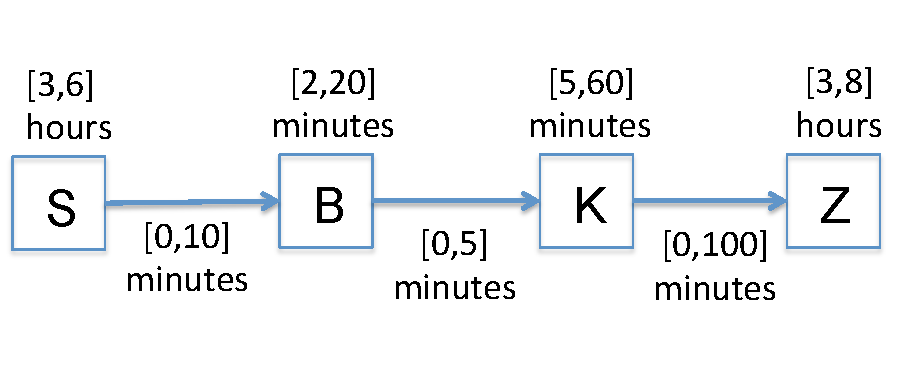
\includegraphics[width=0.5\textwidth]{adlfigs/durationgapconstraint.pdf}
\caption{Example of Duration-gap Constraint Episode.\label{fig_durationgapconstraint}}
\end{figure}

\begin{figure}[!hbtp]
\centering
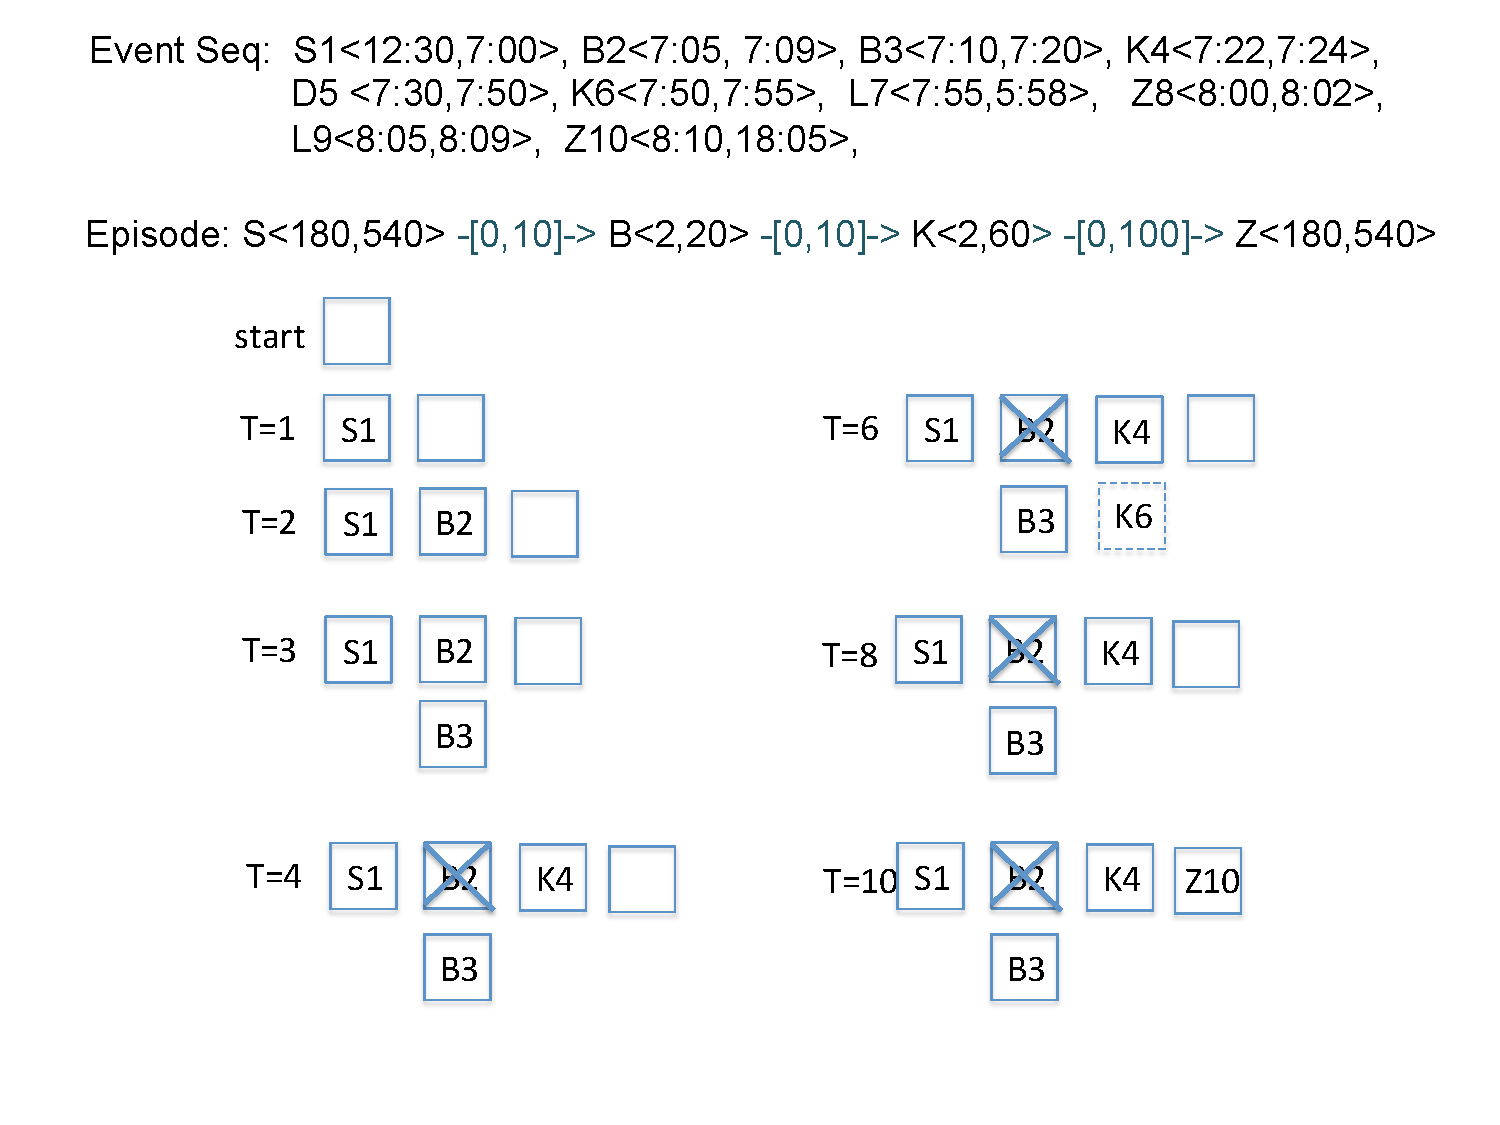
\includegraphics[width=0.5\textwidth]{adlfigs/MingExample.pdf}
\caption{Time-gap constraint episode mining example.\label{fig_MingExample}}
\end{figure}

Figure~\ref{fig_MingExample} shows a time-gap constraint episode mining example. 
Let us assume we have a frequent episode $S\rightarrow B \rightarrow K\rightarrow Z$. 
We must then add the time constraints to each event $\{S,B,K,Z\}$: 
the dwelling duration for $S$ is 3 to 9 hours,   
for $B$ it is 2 to 20 minutes, 
for $K$ it is 2 to 60 minutes, 
and for $Z$ it is 3-9 hours. 
In addition, we must specify the gap duration between any two consecutive events. 
The gap duration of $SB$ is calculated as $\Delta{SB} = B.start-S.end$. 
For example, we set the maximum gap time between SB, BK, and KZ as 
10 minutes, 10 minutes and 100 minutes, respectively; 
the minimum gap time is 0. 
We now have a stream composed of the sequence of dwelling events "Event seq," as shown 
in Figure~\ref{fig_MingExample}.  
 The time-gap constraint episode mining process applied
 to discover a frequent episode uses the following method. 
 Let the $node$ structure denote each element in any episode, 
 depicted as a square box in Figure~\ref{fig_MingExample}.  
Let $waits$ refer to a structure that pairs with an episode 
and has the same length as this episode. 
This creates an initial $waits$ structure related to the episode of $S\rightarrow B \rightarrow K\rightarrow Z$. 
A $node$ structure related to $S$ is created that waits for the first 
element of the episode $S\langle 180, 540 \rangle $. 
When $T=1$, the duration of $S_1$ is checked. 
Since $S_1$ is in the range of $3-9$ hours, 
$S_1$ passes and is put into the node structure $node$ related to $S$. 
Next a new $node$ structure is created to wait for $B\langle 2, 20 \rangle $. 
When $T=2$ and $T=3$, both $B_2$ and $B_3$ 
are qualified in terms of the time constraints and 
the gap constraints; 
this means that the gap between $S$ and $B$ $\Delta SB$ should 
be between 0 and 10 minutes. 
These two nodes $B_2$ and $B_3$ are then input into the 
$waits$ structure. 
At the same time, 
a new $node$ structure is created for $K\langle 2, 60 \rangle $. 
When $T=4$, the gap between $\langle B_3, K_4 \rangle$ 
is satisfied with a distance condition between 
$B$ and $K$ of 0-10 minutes. 
However, the gap between $\langle B_2, K_4 \rangle$ 
is longer than the constraint gap, so $B_2$ is canceled out. 
Now a new $Z$ waits for the symbol $Z\langle 180, 540 \rangle$. 
When $T=6$, the gap from $B_2$ to $K_6$ is 
too large, so $K_6$ is not added into the $node$ $K$ structure in $waits$.
When $T=8$, the duration of $Z_8$ does not satisfy the condition of between 3-9 hours,  
so $Z_8$ is not added, 
but when $T=10$, the duration of $Z_{10}$ does meet the requirement of between 3-9 hours 
and its distance to $K4$ also meets the requirement 
of $\Delta KZ \in [0,100]$ minutes. 
Thus, $Z_{10}$ is added into the $node$ $Z$ structure in $waits$.
The mining of this episode is now complete, and 
we have mined the instance $S_1B_3K_4Z_{10}$. 

%This complete gap-constraint episode mining on dwelling events 
%is described in detail in Algorithm \ref{alg_episodeMiningConstraint}
%\ref{alg_episodeMiningConstraint_2e} 
%in the appendix section.

%Non-overlap episode mining is defined as \textit{Definition}. 
\subsection{Mixture EGH}
\textbf{Episode Generating HMM}
The episode generative HMM (EGH) model is a 
type of HMM that connects frequent episodes, 
and the more frequently an episode occurs inside a sequence, 
the greater the likelihood of the state sequence including that episode~\cite{laxman2008stream}.  
%$\alpha$ with a special HMM model $\Lambda_\alpha$. 
The unique feature of EGH is that 
the transition matrix and 
emission matrix are solely decided by a noise parameter $\eta$. 
The noise parameter $\eta$ of a frequent episode $\alpha$ 
is calculated as $\eta=\frac{T-Nf_{\alpha}}{T}$,  
where $T$ is the training data stream length, 
$\alpha$ is the frequent episode, 
$N$ is the length of frequent episode $\alpha$, 
and $f_{\alpha}$ is the frequency over time $T$.

%% not sure whether should be included 09112015
In the mixture EGH model shown in Figure \ref{fig_egh}, 
the transition matrix for EGH is given as an example. 
Let us assume we have an N-node frequent episode $S\rightarrow B\rightarrow Z$, where $N=3$.
We define 2N hidden states: 
N episode states and N noise states, where
the noise states are $\{W, X, Y\}$. 
An episode state transfers to another episode state 
with a probability of $1-\eta$; 
an episode state transfers to a noise state 
with a probability of $\eta$; 
and a noise state transfers to another noise state 
with a probability of $1-\eta$. 
To calculate the emission matrix, first 
let M denote the total number of symbols in the event stream. 
For any hidden states in the episode, M has a delta function emission. 
Whenever it is visited (right alignment of the first element in the episode, 
left alignment for the left elements in the episode), 
it will generate the same observation symbol. 
For any noise hidden states, it emits any of the symbols from the $M$ 
observation symbols with a uniform distribution at probability $\frac{1}{M}$. 
\begin{figure}[!hbtp]
\centering
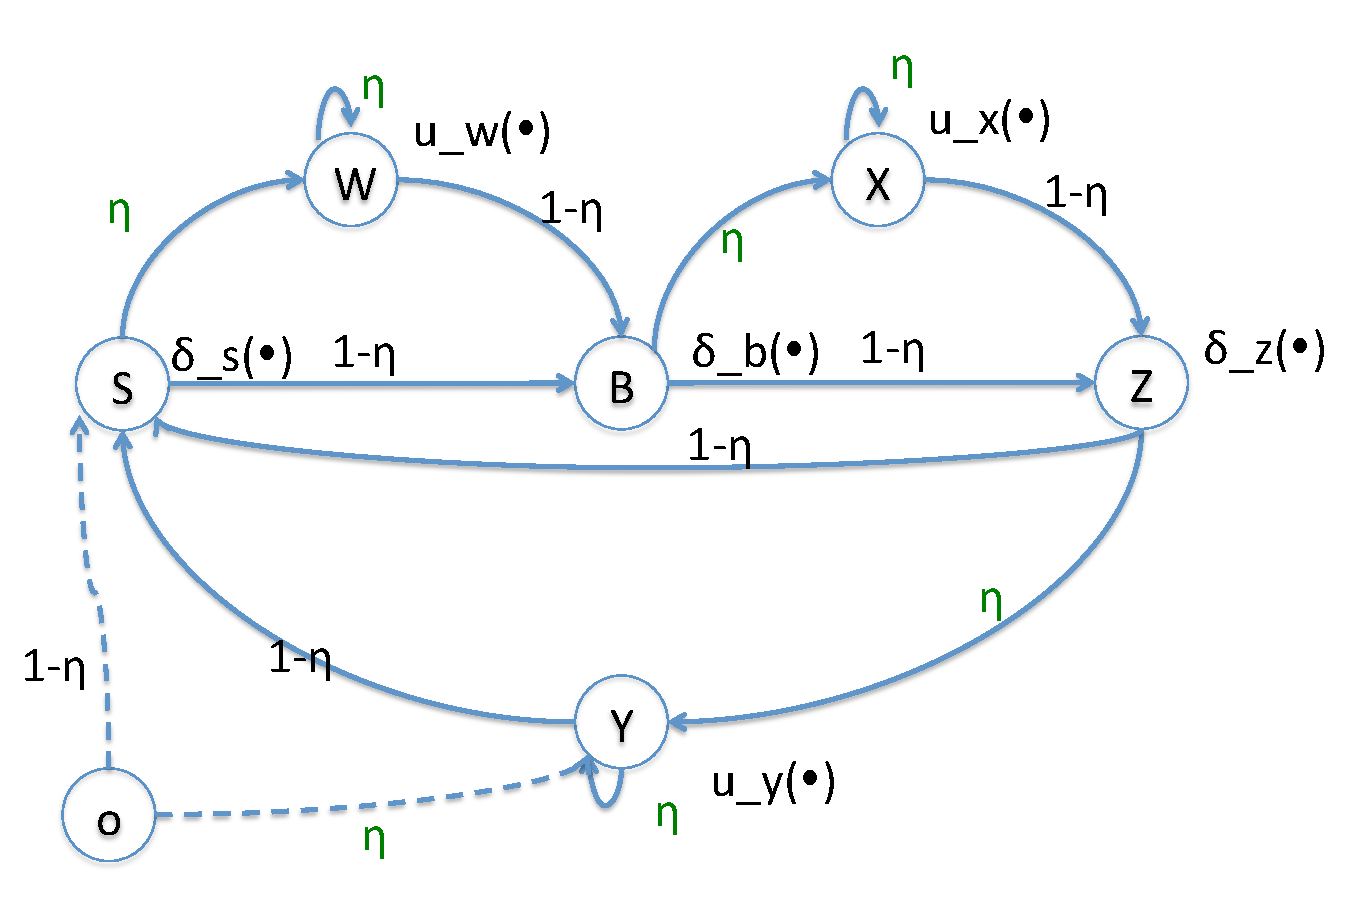
\includegraphics[width=0.5\textwidth]{adlfigs/egh.pdf}
\caption{States Transition of Episode Generating HMM (EGH).\label{fig_egh}}
\end{figure}


Theorem \ref{theorem1} from \cite{laxman2008stream} is crucial here as it
proves that the more frequently an episode occurs within a sequence, 
the greater the likelihood that the state sequence will include this episode. 
The proof for this theorem is explained in detail in \cite{laxman2008stream}. 


\newtheorem{mydef}{THEOREM}
\begin{mydef}
\label{theorem1}~\cite{laxman2008stream} 
Let $D_Z={X_1,..., X_K}$ represent the given sequence data, where $\varepsilon$ is the symbol set, 
and the size of these symbols is $M$. 
Given two frequent N-node episodes $\alpha$ and $\beta$ with frequencies $f_{\alpha}$ 
and $f_{\beta}$, respectively, their corresponding EGH will be $\Lambda_{\alpha}$ and $\Lambda_{\beta}$. 
The most likely state sequences for episodes $\alpha$ and $\beta$ are
$q_{\alpha}^*$ and $q_{\beta}^*$. 
The noise parameters for these two EGH are 
$\eta_{\alpha}$ and $\eta_{\beta}$. 
Assuming that both of these noise parameters are less than $\frac{M}{M+1}$, 
we have 
(1) if $f_{\alpha} > f_{\beta}$, then $P(D_Z, q_{\alpha}^*| \Lambda) > P(D_Z, q_{\beta}^*| \Lambda)  $
(2) if $P(D_Z, q_{\alpha}^*| \Lambda) > P(D_Z, q_{\beta}^*| \Lambda)  $, $f_{\alpha} > f_{\beta}$
\end{mydef}

\textbf{Mixture Model}
The mixture EGH model is fully discussed in previous work \cite{laxman2008stream}, 
which shows how the model 
gives different weights to each EGH
when predicting a target event. 
We can assume we know whether an episode occurs on a certain day. 
Let $D_Z=\{X_1,..., X_K\}$ denote the data set for $K$ days. 
$F=\{\alpha_1, ... \alpha_J\}$ denotes the frequent episodes in the dataset $D_Z$. 
An EGH $\Lambda_{\alpha_j}$ 
is associated with frequent episode $\alpha_j$.
$\Lambda_Z$ denotes a mixture EGH model. 
The likelihood of $D_Z$ under the mixture model is written as Equation (\ref{eq_mixture}).
\begin{eqnarray}
\label{eq_mixture}
Pr(\Lambda|Z) &=& \prod_{i=1}^K P[X_i|\Lambda_Z] \\
			&=& \prod_{i=1}^K ( \sum_{j=1}^J \theta_j P[X_i| \Lambda_{\alpha_j}])
\end{eqnarray}
where $\theta_j$ is the mixture coefficient of $\Lambda_{\alpha_j}$ and is subject to 
$\sum_{j=0}^J \theta_j=1$ 

The parts inside Equation (\ref{eq_mixture}) are additive; 
the coefficients $\theta$ are computed by an EM algorithm. 
%The detailed description is algorithm %%%\ref{alg3} 
%in the appendix section.
%% algorithm 03
\renewcommand{\algorithmicrequire}{\textbf{Input:}}
\renewcommand{\algorithmicensure}{\textbf{Output:}}

\begin{algorithm}
\caption{EM Algorithm for mixture EGH}
\label{alg3}
\begin{algorithmic} [1]
\REQUIRE day episode matrix, 
each element $e_{ij}$ records for each day whether an episode $j$ happens in day $i$;
frequent episodes $F=\{\alpha_1, ..., \alpha_J\}$;
symbol set $\varepsilon$;
threshold $\gamma$

\ENSURE the parameters for mixture EGH $\Lambda_Z=\{  (\Lambda_{\alpha_j}, \theta_j ) , j=1,...,J \}$


\STATE calculate the number of episodes J, and number of days K
\STATE calculate all $\eta$s' threshold value $mThreshold= \frac{M}{M+1}$

\COMMENT{initialize all the thetas to be $\frac{1}{J}$}
\COMMENT{calculate the total frequency for each episode over training time series}
\COMMENT{ calculate the $eta$ value}
\FOR{$0 \leq j \leq J$}
\STATE $\theta[j]= 1/J$
\STATE $episodeFreq[j] = \sum_i^K e_{ij}$
\ENDFOR

\STATE select those frequent episodes starting with 'S' and ending with 'Z' and separate these 
episodes by workday or holiday

\COMMENT {calculate $eta$ for each episode} 
\FOR{$0 \leq j \leq J$}
\STATE $\eta[j]= 1-episodeLen[j]*episodeLen/T$
\ENDFOR

\COMMENT{likelihood prediction of each episode $j$ in the $k$th day}

\FOR{$0 \leq i \leq K$}
\FOR{$0 \leq j \leq J$}
\STATE $likelihood_{ij} = \frac{1-\eta[j]}{\eta[j]/M} ^ {episodeLen[j]*e_{ij}}$
\ENDFOR
\ENDFOR

\COMMENT{calculate the obj value based on J, K, $likelihood_{ij}$ and $\theta$}
\WHILE{$newObj- obj > \gamma$}
\STATE $\theta_{new}=[]$
\FOR{$0 \le l \le J$}
\STATE $temp=0$
\FOR{$0 \le j \le K$}
%\COMMENT{calcuate the new likelihood with Bayes rules}
\STATE $temp = temp+ \frac{\theta_l*likelihood_{il}}{ \sum_0^J { \theta_j*likelihood_{ij}}}$

\ENDFOR
\STATE $\theta_{new}[l] = temp/K $
\ENDFOR

\STATE calculate the newObj
\IF{$newObj-obj > \gamma$}
\STATE $obj=newObj$
\STATE $\theta_{new} = \theta$
\ENDIF

\ENDWHILE

\STATE Output $\Lambda_Z=\{  (\Lambda_{\alpha_j}, \theta_j ) , j=1,...,J \}$

\end{algorithmic}
\end{algorithm}
During the initialization %line 1-10
part of the EM algorithm, 
the episode frequency over the time series T over $K$ days is calculated and 
specific frequent episodes ending with target event 'Z' selected. 
Optionally, 
we could add special constraints on episodes, starting with 
certain types of event 'S'. 
%calculated in lines 11-16. 
% not sure this paragraph to be added or not
In the expectation step, 
one key part is the likelihood value of each episode $\alpha_j$ in time series $X_i$.
The likelihood value is computed as Equation (\ref{eq_likelihood}), after which
Bayes rule is applied to compute the new coefficient $\theta_{new}$. 
\begin{equation}
\label{eq_likelihood}
Pr(X_i| \Lambda_{\alpha_j}) = (\frac{\eta_{\alpha_j}}{M})^{|X_i|} (\frac{1-\eta_{\alpha_j}}{\eta_{\alpha_j}/M})^{|\alpha_j|f_{\alpha_j}(X_i)}
\end{equation}
In the maximization step, 
we update the objective value based on Equation (\ref{eq_mixture}) until it converges, i.e., 
until the difference between two consecutive objective values 
is smaller than a given threshold.%$\gamma$.


\subsection{Predict When the Target Event Occurs}
Although target event prediction has been studied in~\cite{laxman2008stream},  
researchers only sought to predict whether a target event would occur, 
rather than when it would happen. 
Our occupancy prediction algorithm enriches the previous 
event prediction algorithm by breaking it up into three sub-problems: whether the target event un-occupancy $Z$ will appear; when the target event $Z$ will start; and when the target event $Z$ will end. 

Since the solution to the first sub-problem is similar to 
that addressed in previous work, 
this sub-section focuses on the last two sub-problems. 
After obtaining the results for the first sub-problem, 
we can assume we already know that the target event $Z$ will indeed happen, 
and so the next step is to predict when the person will leave or come back. 
The departure time corresponds to the start time of the dwelling event, $Z.start$, and 
the return time refers to the end time of the dwelling event, $Z.end$. 
%This prediction algorithm is described in algorithm \ref{alg22}. 

After running the episode mining algorithm and mixing the EGH model, 
we have obtained all the frequent episodes $F=\langle \alpha_1,..., \alpha_J \rangle$, 
the corresponding EGH $\Lambda_{\alpha_j}, j=1...J$ with noise parameter $\eta_j$, 
and the mixture models $\Lambda_Z$ with coefficients $\theta_j$.
We can use the coefficient of these mixture models to predict the departure and return times for
target event $Z$. 
 Each day is separated into three phases: 1) before a person gets up; 
2) after the person has got up but before he/she goes out;
and 3) after the person goes out but before he/she comes back. 
\begin{enumerate}
\item
Usually before a person gets up, there is only one frequent episode, namely 'SZ'. 
The start time and end time of $Z$ depends on 'S'. 
Therefore $Z.start$ and $Z.end$  are calculated based on the probability density function of 
the departure and return times for previous days. 
\item
After the person gets up, if he/she has engaged in a number of activities at home, 
several frequent episodes will be mined before the person leaves home. 
If there are several frequent episodes ending with $Z$,  
the leave time and return time of each episode is checked to determine
whether they fall within the range of probability density function (PDF) values observed previously. 
If the answer is yes, the mean value of these episodes is recorded. 
Since each episode generates an EGH, 
the mixture EGH model computes a weight for each EGH as a coefficient. 
The departure time $Z.start$ and return time $Z.back$ are 
the weighted mean departure and return times of these frequent episodes. 
\item
After a person has left home, 
we already know when the departure time $Z.start$. 
If the person has come back
nothing needs to be predicted, but 
if the person has not come back,  
the return time $Z.end$ is the weighted 
 historical return time of the mined 
frequent episodes, 
viz. the probability density function of the return time is based on the 
time-constraint for the departure.
\end{enumerate}

\iffalse
The algorithm \ref{alg22} 
uses partial day of test data $s$, 
all the frequent episodes  $epis$, 
the frequent episodes $F$ in partial day of $s$, 
the mixture model $\Lambda_Z$, 
to predict when the person leaves or comes back home. 
The partial day is cut by partial index $pIndex$. 
Each day is cut into three phases, before the person gets up; 
after the person gets up but before the person leaves home;
after the person comes back home. 

In the first two phases, before the person leaves, 
the PDF leave time and back time are calculated from line 2-4. 
Usually before a person gets up, there is only one frequent episode named 'SZ'. 
After the person gets up, he/she has a lot of activities at home, 
there are several frequent episodes mined before the person leaves home. 
In case there are several frequent episodes in lines 6-12, 
the leave time and back time of each episode is checked
whether they are in a range of PDF value in the past. 
If yes, the mean value of these episodes are recorded from line 14-17. 
If there are several frequent episodes with corresponding EGH, 
the leave time $Z_{leave}$ and back time $Z_{back}$ is the weighted 
mean leave time and back time of each episode in lines 18-21. 

In the third phase, after the person leaves home, 
we already know when the person leaves home $Z_{leave}$ 
but needs to predict when the person comes back $Z_{back}$. 
If the person has come back, that means $Z_{back}$ is not equal to $Z_{leave}$. 
We don't need to do anything. 
If the person has not come back, that means $Z_{back}$ equals to $Z_{leave}$. 
The back time is the past weighted back time from line 28-34. 
%% algorithm 22, an extention of algorithm 2
\renewcommand{\algorithmicrequire}{\textbf{Input:}}
\renewcommand{\algorithmicensure}{\textbf{Output:}}

\begin{algorithm}
\caption{ Target Event Occurs Time Prediction Algorithm}
\label{alg22}
\begin{algorithmic} [1]
\REQUIRE 
partial day cut point $pIndex$, $s[1:pIndex]$ is known,  and $s[pIndex:96]$ for prediction;
partial day event stream $s=\langle E_1,..., E_{pIndex} \rangle$;
all the episodes $epis$, $\forall E \in \alpha$ and $\forall \alpha \in epis$, E has $E.{start}$ 
and $E.{end}$; 
frequent episodes $F=\langle \alpha_1,..., \alpha_J \rangle$ inside $s[1:pIndex]$;
EGH model $\Lambda_{\alpha_j}$ with noise parameter $\eta_j$ where $j=1...J$
EGH mixture model coefficients $\Theta=\langle \theta_1,...,\theta_J \rangle$;
the slot number noise parameter $\epsilon$  ; 
target event $Z$
\ENSURE Predict target event leaving time $Z_{leave}$ and back time $Z_{back}$
 
\IF{$Z  \notin s $}%\COMMENT{predict before the person leaves home}
\STATE choose episodes $\alpha.ev={'SZ'}$ 
\STATE $Z_{leave} = \frac{\sum_1^K Z.start}{|\alpha|} $
\STATE $Z_{back} = \frac{\sum_1^K  Z.end}{|\alpha|}  $
\IF{$len(F)>1$}%\COMMENT{if there are several episodes to predict 'Z'}
\FOR{$\alpha_j \langle e_1,..., e_j \rangle \in F$}
%\IF{$\alpha_j.ev='SZ'$} % 'SZ' has been calculated,no need to calculate again
%\STATE break
%\ENDIF
\IF{$pIndex \in ( \alpha_j. ev[-2].start - \epsilon, \alpha_j.ev[-2].start+ \epsilon )$}
\STATE $leaveMap[\alpha_j.ev]=\alpha_j.leave$
\ENDIF
\IF{$pIndex \in ( \alpha_j. ev[-2].end - \epsilon, \alpha_j.ev[-2].end+ \epsilon )$}
\STATE $backMap[\alpha_j.ev]=\alpha_j.back$
\ENDIF 
\ENDFOR
\IF{$len(leavingMap) !=0 $} % for the average
\STATE $leaveSlotMap[\alpha_j.ev] =\frac{\sum_1^K leavingMap.get(k)}{K}$
\STATE $backSlotMap[\alpha_j.ev] = \frac{\sum_1^K backMap.get(k)}{K}$
\ENDIF % this is for the len\\
\IF{$K=len(leaveSlotMap)>1$}%\COMMENT{There are other frequent episodes except 'SZ'}
\STATE $Z_{leave}= \frac { \sum_{k=1}^K leaveSlotMap.get(k) * \theta_k } {K}$
\STATE $Z_{back}= \frac { \sum_{k=1}^K backSlotMap.get(k) * \theta_k } {K}$
\ENDIF
\ENDIF %this is for len(F)>1 
\ENDIF %this is for if Z \notin S \\
\IF{$Z  \in s $}%\COMMENT{if the person has left home}
\STATE $Z_{leave}=s.firstindex[Z]$ % the position where $Z$ first appears
\STATE $Z_{back}=s.lastindex[Z]$ % the position when $Z$ lastly appears\\
%\STATE backSlotMap=\{\}
\IF{$Z_{leave}=Z_{back}$} %\COMMENT{The person hasn't come back}% the person hasn't come back
% get the average of those time
\FOR{$\alpha_j \langle e_1,..., e_j \rangle \in F$}
\IF{$Z_{leave} \in [\alpha_j.ev[-2].end - \epsilon, \alpha_j.ev[-2].end + \epsilon ]$}
\STATE $backSlotMap[\alpha_j.ev] = \alpha_j.leave$
\ENDIF
\ENDFOR
\STATE $Z_{back}= \frac { \sum_{k=1}^K backSlotMap.get(k) * \theta_k } {K}$
\ENDIF
\ENDIF
\STATE Output the slot number when the person leaves $Z_{leave}$ and comes back $Z_{back}$
\end{algorithmic}
\end{algorithm}
\fi

 





